\documentclass{article}
\usepackage[utf8]{inputenc}
\usepackage{amsmath,graphicx,hyperref,xcolor}

\setlength{\parindent}{0in}
\setlength{\parskip}{1em}

\usepackage{fancyhdr}

\rhead{}
\lhead{Guides and tutorials}

\pagestyle{fancy}
\lhead{Physics 374B Quiz 1}
\rhead{Fall 2020}
\cfoot{\thepage}

\newcommand{\purple}[1]{{\color{purple} #1}}

\begin{document}

Name: \makebox[2in]{\hrulefill\purple{SOLUTION}\hrulefill}

\vspace{0.5in}

\begin{itemize}
    \item Begin at 10:45am. Return your answers by 11:45am via email. 
    \item Work on your own. Do not refer to any outside materials such as notes, homework, or the text.
    \item Please join the Zoom meeting. I will put you each in your own breakout room. You do not need to be on screen. To ask a question, use the ``Ask for help" button. If it takes me more than a minute or two to show up, try again. Sometimes Zoom gets confused.
    \item Each bullet point is worth the same amount. They are not all equally difficult. You do not need to complete them in order.
    \item After you're done, drop off your quiz in Regents. There will be an envelope outside Darla's office (RNS 236) until 3pm. This is so she can send me scans in case photos are not legible. Make sure your name is on every page!
    \item I have confidence in you!
\end{itemize}

\vfill

I pledge my honor that on this examination I have neither given nor received assistance not explicitly approved by the professor and that I have seen no dishonest work \makebox[2in]{\hrulefill}

\vspace{0.5in}

I have intentionally not signed this pledge \makebox[2in]{\hrulefill}

\newpage

\section*{Problem 1}

The event horizon of a black hole is the point beyond which gravity is so strong that nothing can escape -- not even light. We are interested in using dimensional analysis to express the radius of the event horizon in terms of the gravitational constant $G$, the black hole mass $M$, and/or the speed of light $c$. 

\begin{itemize}
    \item Show that the units of $G$ are $[length]^3 [mass]^{-1} [time]^{-2}$
    Hint: The gravitational force between two objects is given by $F = G\frac{m_1 m_2}{r^2}$, where $m_1$ and $m_2$ are masses and $r$ is the distance between them.
    
    \purple{
    Force has units of $[mass][length][time]^{-2}$. So:
    $$
    [mass][length][time]^{-2} = G \, [mass]^2 [length]^{-2}
    $$
    So $G$ must have units of $[mass]^{-1} [length]^{3} [time]^{-2}$
    }
    \item Suppose $R = G^{\alpha} M^{\beta} c^{\gamma}$, then write down a system of linear equations relating $\alpha$, $\beta$, and $\gamma$. 
    
    \purple{
    $G$ has units of $[mass]^{-1} [length]^{3} [time]^{-2}$.
    
    $R$ has units of $[length]$.
    
    $c$ has units of $[length][time]^{-1}$.
    
    $M$ has units of $[mass]$. 
    
    So if:
    $$
    R = G^\alpha M^\beta c^\gamma
    $$
    Then in terms of units:
    $$
    [length] = [length]^{3\alpha} [mass]^{-\alpha} [time]^{-2\alpha} \; [mass]^\beta \; [length]^\gamma [time]^{-\gamma}
    $$
    Or, breaking each unit out into its own equation:
    \begin{align*}
        [length]^{1} &= [length]^{3 \alpha} \; [length]^{\gamma} \quad &\rightarrow \quad 1 &= 3\alpha + \gamma \\
        [mass]^0 &= [mass]^{-\alpha} \; [mass]^\beta \quad &\rightarrow \quad 0 &= -\alpha + \beta \\
        [time]^0 &= [time]^{-2\alpha} \; [time]^{-\gamma} \quad &\rightarrow \quad 0 &= -2\alpha - \gamma \\
    \end{align*}
    }    
    \item Solve the system of equations to write $R$ in terms of $G$, $M$, and/or $c$
    
    \purple{
    The second equation shows $\alpha=\beta$. From there it's straightforward to end up with $\alpha=\beta=1$ and $\gamma=-2$. So:
    $$
    R = \frac{GM}{c^2} 
    $$
    }
    \item Does this solution make sense? What would happen if the black hole gained mass, or if the speed of light got faster?
    
    \purple{
    A bigger $R$ means that the black hole ``reaches" further. Small $R$ is easier to escape, since you have to be closer to ``fall in" to the black hole.
    
    As $M$ increases, the black hole gets bigger, reaches further. This makes sense, since we know heavier things pull harder.
    
    As $c$ increases, the radius of the black hole decreases. Another way to think about this is that it's harder to trap things that are moving faster.
    }
\end{itemize}

\newpage

\section*{Problem 2}

Consider a cone with constant slope $\lambda$. The relationship between Cartesian coordinates and cone coordinates is:
$$
x=\rho \sin\phi
\quad \quad 
y=\rho \cos\phi
\quad \quad
z=\lambda\rho
$$

\begin{itemize}
    \item Show that the expression for a small path $d\ell$ along the surface of the cone is given by:
    $$
    d\ell = \sqrt{ \left( 1 + \lambda^2 \right) d\rho^2 + \rho^2 d\phi^2}
    $$
    
    \purple{
    Getting a differential element for each Cartesian dimension, using the product rule. For example:
    $$
    dx = \frac{dx}{d\rho} d\rho + \frac{dx}{d\phi} d\phi
    $$
    Note $\lambda$ is constant, $\rho$ and $\phi$ are not.
    \begin{align*}
        dx &= \rho \cos\phi \, d\phi + \sin\phi \, d\rho \\
        dy &= -\rho \sin\phi \, d\phi + \cos\phi \, d\rho \\
        dz &= \lambda \, d\rho
    \end{align*}
    When we square those all and plug them into $d\ell = \sqrt{ dx^2 + dy^2 + dz^2}$, the mixed terms ($d\rho \, d\phi$) cancel out and we end up with the expected expression.
    }
    \item Let $(\rho_1, \phi_1)$ and $(\rho_2, \phi_2)$ be two points on the surface of the cone, neither of which is the tip. Show that a path from $(\rho_1, \phi_1)$ to $(\rho_2, \phi_2)$ can be written:
    $$
    \ell = \displaystyle \int_{\rho_1}^{\rho_2} d\rho \sqrt{1 + \lambda^2 + \rho^2 \phi'^2}
    \quad \mathrm{where} \quad
    \phi' = \frac{d\phi}{d\rho}
    $$
    
    \purple{
    To get the length of the path from $A$ to $B$, integrate our differential length elements:
    $$
    \ell = \displaystyle\int_{\rho_1, \phi_1}^{\rho_2, \phi_2} d\ell = \displaystyle\int_{\rho_1, \phi_1}^{\rho_2, \phi_2} \sqrt{ \left( 1 + \lambda^2 \right) d\rho^2 + \rho^2 d\phi^2 }
    $$
    Say $\rho$ is our independent variable and $\phi = \phi(\rho)$. Then factor $d\rho$ out of the expression:
    $$
    \ell = \displaystyle\int_{\rho_1}^{\rho_2} d\rho \; \sqrt{ \left( 1 + \lambda^2 \right) \left( \frac{d\rho}{d\rho} \right)^2 + \rho^2 \left( \frac{d\phi}{d\rho} \right)^2 } = \displaystyle\int_{\rho_1}^{\rho_2} d\rho \; \sqrt{ \left( 1 + \lambda^2 \right) + \rho^2 \phi'^2 }
    $$
    }
    \item In the above expression, we have chosen $\rho$ as the independent variable and written $\phi = \phi(\rho)$. Why might that be more convenient than the other way around?

    \purple{
    Our integrand does not include $\phi$ -- only $\phi'$. That means the $\frac{\partial f}{\partial \phi}$ term in the Euler-Lagrange equation is zero. The integrand does include $\rho$, so if we had done things the other way around, none of our terms would be zero.
    }
    \item Let $\phi(\rho)$ describe a path from $(\rho_1, \phi_1)$ to $(\rho_2, \phi_2)$. Show that the length of that path is minimized when $\phi(\rho)$ satisfies the following differential equation:
    $$
    \frac{d\phi}{d\rho} = \frac{k}{\rho^2} \frac{\sqrt{1 + \lambda^2} }{\sqrt{1 - \left( \frac{k}{\rho} \right)^2}}
    \quad \quad 
    \text{where $k$ is a constant}
    $$
    Hint: the Euler-Lagrange equation for $f(\phi, \phi', \rho)$ is \; $\frac{\partial f}{\partial \phi} - \frac{d}{d \rho} \left( \frac{\partial f}{\partial \phi'} \right) = 0$
    
    \purple{
    Our integrand $f$ is:
    $$
    f(\phi, \phi', \rho) = \sqrt{ \left( 1 + \lambda^2 \right) + \rho^2 \phi'^2 }
    $$
    To minimize it, we'll plug it into the Euler-Lagrange equation. First up, evaluate a few derivatives:
    $$
    \frac{\partial f}{\partial \phi} = 0
    \quad \quad \text{and} \quad \quad
    \frac{\partial f}{\partial \phi'} = \frac{\rho^2 \phi'}{\sqrt{ \left( 1 + \lambda^2 \right) + \rho^2 \phi'^2 }}
    $$
    Plugging into the Euler-Lagrange equation:
    $$
    0 - \frac{d}{d\rho} \left( \frac{\rho^2 \phi'}{\sqrt{ \left( 1 + \lambda^2 \right) + \rho^2 \phi'^2 }} \right) = 0
    $$
    In other words:
    $$
    \frac{\rho^2 \phi'}{\sqrt{ \left( 1 + \lambda^2 \right) + \rho^2 \phi'^2 }} = k \quad \text{(constant)}
    $$
    A bit of algebra...
    \begin{align*}
        \rho^2 \phi' &= k \sqrt{ \left( 1 + \lambda^2 \right) + \rho^2 \phi'^2 } \\
        \rho^4 \phi'^2 &= k^2 \left( \left( 1 + \lambda^2 \right) + \rho^2 \phi'^2 \right) \\
        \phi'^2 \left( \rho^4 - k^2 \rho^2 \right) &= k^2 \left( 1 + \lambda^2 \right) \\
        \phi'^2 &= \frac{k^2 \left( 1 + \lambda^2 \right) }{\left( \rho^4 - k^2 \rho^2 \right)} \\
        \phi' &= \frac{k}{\rho} \frac{\sqrt{ 1 + \lambda^2 } }{ \sqrt{ \rho^2 - k^2 } } = \frac{k}{\rho^2} \frac{\sqrt{ 1 + \lambda^2 } }{ \sqrt{ 1 - \frac{k^2}{\rho^2} } }
    \end{align*}
    }
    
    \item Separate and solve the above differential equation. Show the result is:
    $$
    \phi(\rho) = \phi_0 + \sqrt{1 + \lambda^2} \cos^{-1} \left( \frac{\rho_0}{\rho} \right)
    $$
    Or, if you prefer:
    $$
    \rho(\phi) = \frac{\rho_0}{ \cos \left( \frac{\phi - \phi_0}{ \sqrt{1 + \lambda^2} } \right) }
    $$
    Hint: try the substitution $\cos(u) = \frac{k}{\rho}$
    
    \purple{
    From above:
    $$
    \frac{d\phi}{d\rho} = \frac{k}{\rho^2} \frac{\sqrt{ 1 + \lambda^2 } }{ \sqrt{ 1 - \frac{k^2}{\rho^2} } }    
    $$    
    Which separates to:
    $$
    d\phi = \frac{k}{\rho^2} \frac{\sqrt{ 1 + \lambda^2 } }{ \sqrt{ 1 - \frac{k^2}{\rho^2} } } \, d\rho
    $$    
    We have $\sqrt{ 1 - \text{stuff}^2 }$ in the denominator which suggests a trig substitution. Let's try:
    $$
    \cos u = \frac{k}{\rho} 
    \quad \text{so} \quad
    -\sin u \, du = -\frac{k}{\rho^2} d\rho
    $$
    Plugging that in and integrating to solve:
    \begin{align*}
        d\phi &= \frac{k}{\rho^2} \frac{\sqrt{ 1 + \lambda^2 } }{ \sqrt{ 1 - \frac{k^2}{\rho^2} } } \, d\rho \\
        d\phi &= \sqrt{ 1 + \lambda^2 } \frac{ \sin u  }{ \sqrt{ 1 - \cos ^2 u } } \, du = \sqrt{ 1 + \lambda^2 } \, du \\
        \int d\phi &= \sqrt{ 1 + \lambda^2 } \int du \\
        \phi + C &= \sqrt{ 1 + \lambda^2 } \, u = \sqrt{ 1 + \lambda^2 } \, \cos^{-1}\left( \frac{k}{\rho}\right)
    \end{align*}
    This is perhaps easier to visualize if we invert it to write $\rho(\phi)$.
    $$
    \rho(\phi) = \frac{\rho_0}{ \cos \left( \frac{\phi - \phi_0}{ \sqrt{1 + \lambda^2} } \right) }
    $$
    Here, we have subbed in $k \rightarrow \rho_0$ and $C \rightarrow \phi_0$. The path we're looking at is a line ``draped over" the cone's surface. The point $(\rho_0, \phi_0)$ is the closest point on the curve to the tip of the cone. 
    
    Another way to picture it: consider the endpoints share the same value of $\rho$ (and thus $z$). We might suspect that the quickest way to get from one to the other is to draw a line horizontally between them. But it turns out, we can shorten the line by traversing up the cone, then back down, rather than going all the way around. 
    
    \centering{
    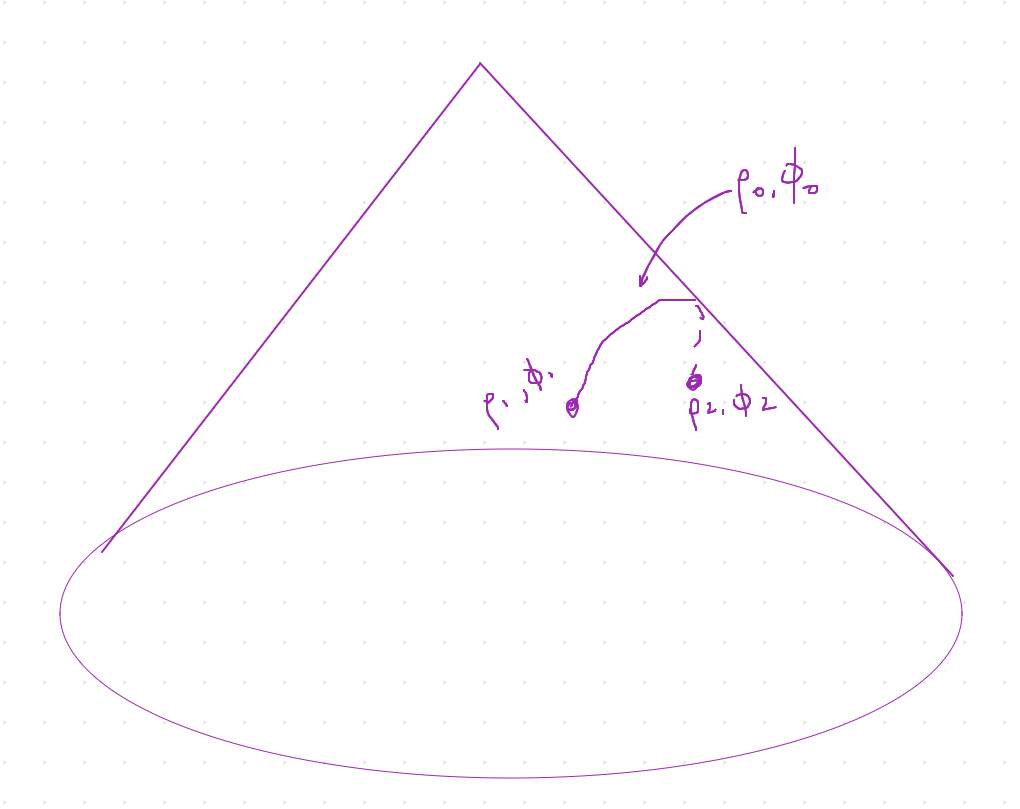
\includegraphics[width=10cm]{cone-path.png}
    }
    }
    \item Discuss the limiting case where $\lambda \rightarrow 0$. Does this solution make sense?
    Hint: in polar coordinates, a straight line on a plane takes the form:
    $$
    \rho(\phi) = \frac{\rho_0}{ \cos \left( \phi - \phi_0 \right) }
    $$

    \purple{
    As $\lambda \rightarrow 0$, the cone gets shorter and shorter, eventually looking like a flat plane. In that case, the solution is a straight line, as we expect.
    
    We may also note that the limit $\lambda \rightarrow \infty$ corresponds to the cone looking like a cylinder. This limiting case is beyond the scope of the quiz, as the math gets a bit tricky.
    }



\end{itemize}

\end{document}
